\setchapterimage[6.5cm]{Grid_FullView_Logo}
\setchapterpreamble[u]{\margintoc}
\chapter{Likelihood Analysis in IceCube}
\labch{llh}
\begin{fquote}[Isaac Asimov][Lady Windermere's Fan][18??] A hypothesis may be simply defined as a guess. A scientific hypothesis is an intelligent guess. 
\end{fquote}
Neutrino Astronomy with IceCube is rather distinct from more mature branches of astronomy, because we have much less power to distinguish astrophysical signal from background. This regime is to some extent fixed by the raw event rate, in which irreducible atmospheric backgrounds are overwhelmingly dominant over astrophysical neutrinos except at the highest energies. However, it is exacerbated by the limited angular resolution of the detector, where each IceCube event covers a relatively-large area of the sky. Further, owing to the limited effective area of IceCube, there are insufficient numbers of signal-like neutrinos to form cleanly-identifiable clusters. Fundamentally, there is almost no signature in data for which a background origin can be discounted.

It is thus not difficult to find interesting things that are correlated with neutrino arrival directions or times, such as weekends or star signs, because any individual hypothesis will have a small probability to be correlated with  neutrinos by chance. The sum of these many small probabilities can become a large probability, and unless we are careful to correct for this look-elsewhere effect, many spurious correlations will be found. To shield against this, anisotropies in neutrino data are studied through \emph{blind analysis}, in which methods are first developed using simulated datasets. Once an analysis method and hypothesis has been finalised, and the procedure for determining the significance of a result has been fixed, the analysis can then be repeated on real data.

A software designed to perform unbinned likelihood analysis, \emph{\href{https://github.com/IceCubeOpenSource/flarestack}{Flarestack}}, was developed by the author to study correlations in IceCube data \sidecite{flarestack}.

\section{Hypothesis Testing}
Statistical hypothesis testing begins with the definition of a particular hypothesis to test, $\mathcal{H_{1}}$, and a null hypothesis, $\mathcal{H_{0}}$, that would be expected in the absence of any correlation. Ultimately, we wish to determine which hypothesis better describes our data. Hypothesis testing begins from the default position that the null hypothesis describes the data, and evaluates whether this description can be disproven. We define a test statistic (TS) to quantify the how well data is described, and define a threshold at which we would be confident in reaching a conclusion. If our test statistic exceeds this threshold, we \emph{reject the null hypothesis}. This means we are confident that the null hypothesis does not describes our data. It does not necessarily follow that our signal hypothesis is correct, we can only say that it better describes our data than the null hypothesis. Conversely, if the TS does not exceed the threshold,  we \emph{do not reject the null hypothesis}. In this case, we are not confident that the null hypothesis does not describe our data. This does not mean that the signal hypothesis is wrong, but rather that we cannot be sure the null hypothesis is wrong. 

\begin{margintable}
	\caption[]{Hypothesis Testing}
	\raggedright
	\begin{tabular}{ c|  c c}
		\hline
		& not rejected & rejected \\
		\hline
		$\mathcal{H_{0}}$ true & \checkmark & Type I \\
		$\mathcal{H_{0}}$ false &Type II & \checkmark\\
		\hline
	\end{tabular}
	\label{tab:hypothesis}
\end{margintable}

As illustrated in Table \ref{tab:hypothesis}, there are two things that can go wrong with a hypothesis test. Type 1 error, or a false positive, occurs when we reject the null hypothesis although it is true. Type 2 error, or a false negative, occurs when we do not reject the null hypothesis even though it is false. By construction, every test must balance the risk of Type 1 and Type 2 errors, and both cannot be eliminated simultaneously. We typically construct our test by fixing a threshold for acceptable rate of Type 1 error. This Type I error rate is quantified by a \emph{p-value}, defined as the probability of observing a result under the null hypothesis that is at least as significant as the one found. One common p-value threshold is 0.05, i.e only accepting results with a probability <5\% to arise under the null hypothesis. The p-vaue can also be converted to a \emph{significance}, equal to the number of standard devations required for a one-sided Gaussian distribution to yield that p-value. A typical threshold for a discovery is $5 \sigma$, corresponding to a p-value of less than $3 \times 10^{-7}$.

In IceCube, null hypothesis rejection is a continuous rather than discrete process. The degree of rejection is parameterised by an informal sliding verbal scale from \emph{hints} ( $\gtrsim 2 \sigma$), through \emph{evidence} ($\gtrsim2.5 \sigma$) and \emph{compelling evidence} ($\gtrsim3 \sigma$), to \emph{discovery} ($\gtrsim5 \sigma$). At discovery, the null hypothesis is considered fully rejected.

While the simplest hypothesis test is a binary case is which one well-defined hypothesis $\mathcal{H_{1}}$ is compared to the null hypothesis, the procedure is often generalised to cover multiple hypotheses, $\mathcal{H_{i}}$, which can be either discrete or continuous. We pick the hypothesis with the smallest p-value, and compare that to our null hypothesis. It is at this point that the look-elsewhere effect from must be accounted for, through use of a trial correction. 

\section{Likelihoods and Wilk's Theorum}

One method of quantifying agreement between a hypothesis and data is to calculate the \emph{likelihood}, $\mathcal{L}$, of observing our data given that hypothesis. For each hypothesis, we can construct probability density functions (PDFs) describing how we would expect data to be distributed for that case. We can then calculate the conditional probability, $\mathcal{L}(x | \mathcal{H})$, of observing our data $x$ given that hypothesis. A common test statistic, used for IceCube analyses, is the log likelihood ratio:

\begin{equation}
TS (\mathcal{H_{i}}) = 2 \log \left( \frac{\mathcal{L}(x | \mathcal{H_{i}})}{\mathcal{L}(x | \mathcal{H_{0}})} \right)
\end{equation}

The primary motivation for this is the \emph{Neyman-Pearson Lemma} \sidecite{1933RSPTA.231..289N}, which states that the likelihood ratio test is the most powerful possible statistical test. This definition is also particularly convenient, because we can analyse the results using \emph{Wilk's Theorum} \sidecite{Wilks:1938dza}. Wilk's Theorum states that the log likelihood ratio for an ensemble of datasets will be distributed according to a $\chi^{2}$ distribution, with degrees of freedom equal to the number of independent parameters. Thus, for a hypothesis depending on a known number of independent parameters, we can convert any TS value to a \emph{p-value}. Even if the number of independent parameters is not known, it can be derived through fits to a sample of pseudodatasets, and then extrapolated to smaller p-values. In this way, a 5$\sigma$ threshold can be calculated without requiring $\sim$several million datasets to be tested.

There is, however, a caveat to Wilk's Theorum. The full formulation only applies in the limit of large samples. In IceCube this condition is usually satisfied, but there are exceptions particularly for searches on short-timescales relevant for GRB or FRB searches, where the data transitions from a background-dominated one to a background-free regime. In such cases, p-values must be derived directly from pseudo-experiments. 

Bounds -> gamma

\section{Null Hypothesis and Background Modelling}

At the stage of defining hypotheses, IceCube-specific physics is added to the pure mathematical basis of hypothesis testing. As outlined in Chapter \ref{ch:event_selection}, IceCube data in the northern hemisphere is dominated by atmospheric neutrinos, while events in the southern hemisphere are dominated by atmospheric muon bundles, and in both hemispheres the signal is subdominant. It is common in IceCube to take the simplifying assumption that \emph{the data is sufficiently background-dominated to be used as a null hypothesis}. The motivation is twofold, it is firstly approximately true, but more importantly the colossal muon rate makes it very difficult to simulate the small fraction of muons which form a signal-like background for the southern hemisphere. In the absence of any adequate simulated model for background in the southern hemisphere, we are forced to instead use a data-based model as a null hypothesis.

The simplification has a number of drawbacks, primarily that PDFs derived from data are necessarily coarser because the available statistics are limited. An alternative approach that for the sample of northern through-going muons tracks, in which there is negligible atmospheric muon background, is to use Monte-Carlo based modelling to construct a model for background. This ultimately introduces the risk of data-MC disagreement,  with uncertainties introduced for example with by atmospheric flux modelling. However, this is typically offset by the high-resolution PDFs which can be constructed using these much larger sample sizes.

In either case, distributions are then constructed for the background model $\mathcal{B}$. It is typical in IceCube to consider event arrival direction, energy and arrival time as key observables to distinguish signal from background. These distributions form our null hypothesis. 

In the following, data-based background PDFs are illustrated for the all-sky \emph{ps tracks version v003-p02} dataset \sidecite{2020PhRvL.124e1103A}.

Distributions based on detector observables.

\begin{equation}
\mathcal{B} (\theta) = \mathcal{B}_{space} \times \mathcal{B}_{time}  \times {B}_{E}
\end{equation}

\subsection{Background Spatial PDF}

\begin{marginfigure}
	\centering 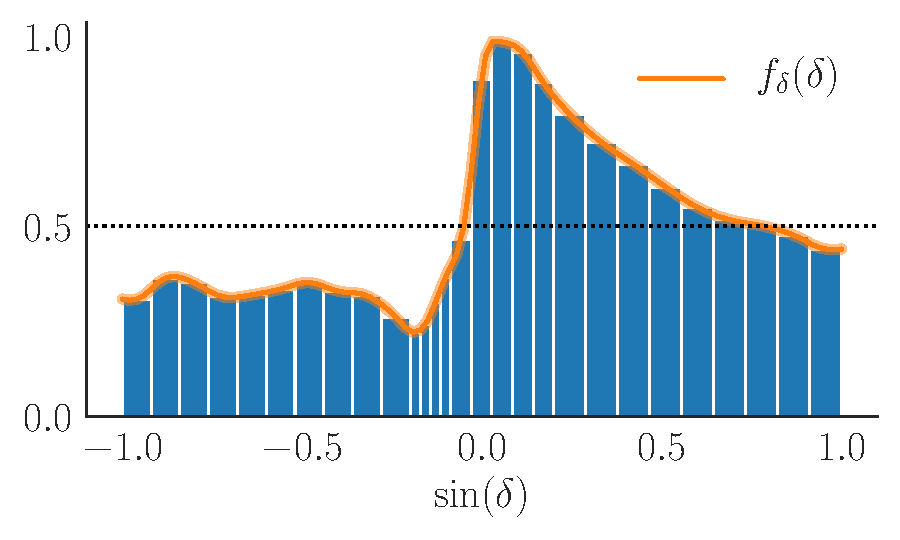
\includegraphics{llh/sindec}
	\caption{Event rate as a function of $\sin(\delta)$.}
	\label{fig:sindec}
\end{marginfigure}

Owing to IceCube's convenient location at the geographic south pole, detector coordinates are uniquely mapped to geometric coordinates. Thus, IceCube's zenith-dependent instrument response is translated into a declination-dependent one which does not change over time. From the background rate, a spatial PDF as a function of declination $ f(\delta)$ can be derived, as seen in Figure \ref{fig:sindec}.

\begin{equation}
	\mathcal{B} (\delta) = f(\delta)
\end{equation}

\begin{marginfigure}
	\centering 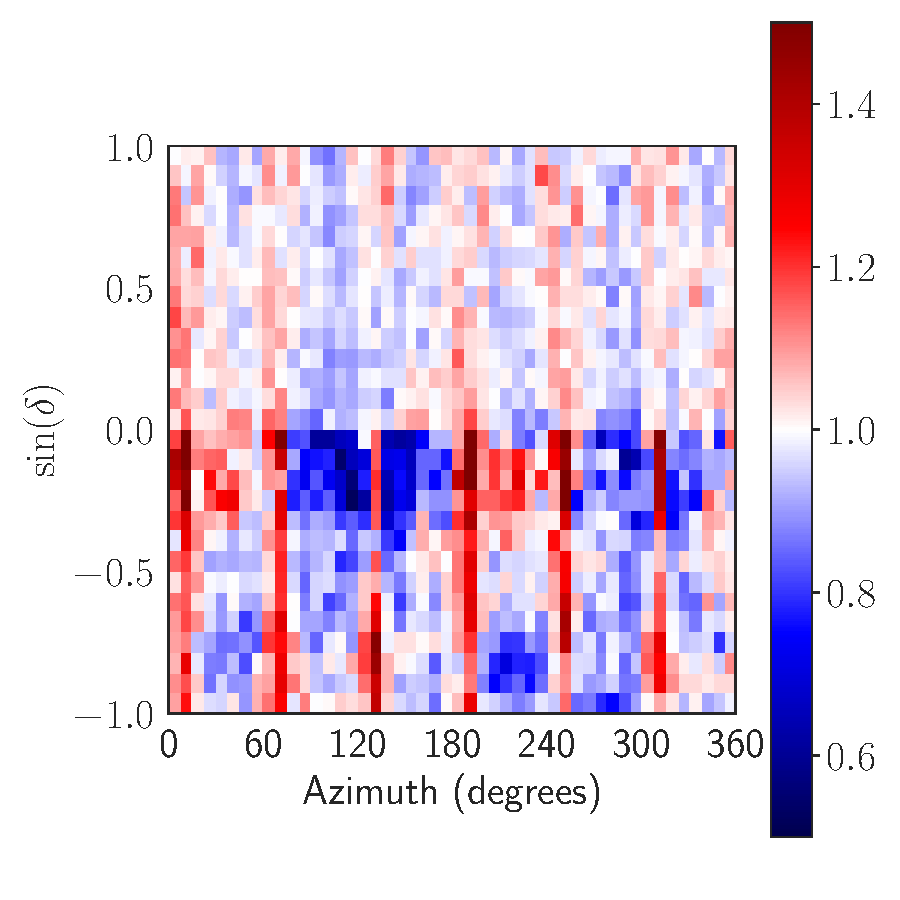
\includegraphics{llh/azimuth}
	\caption{Declination-normalised event rate as a function of azimuth.}
	\label{fig:azimuth}
\end{marginfigure}

Furthermore, IceCube's detector response is assumed, to first order, to be uniform in right ascension.

\begin{equation}
\mathcal{B} (\theta) = \frac{1}{2\pi} 
\end{equation}

More precisely, it is assumed that \emph{any variations due to azimuthal asymmetry are negligible}. The detector itself (see Chapter N) has 6 string axes which will be traced out over the course of each day. Thus, for typical data periods of many years, these azimuthal variations will indeed be negligible. However, particularly in cases which search for clustering over short time periods, this azimuthal asymmetry may have an impact. The degree of azimuthal asymmetry in event rate is shown in Figure \ref{fig:azimuth}.  The six string axes are clearly visible with elevated event rates, reaching $\sim40\%$ variations for the southern hemisphere.

\begin{equation}
\mathcal{B} (\theta, \delta) = \frac{1}{2\pi} \times f(\delta)
\end{equation}


Additionally, the impact of \emph{ice anistropy} can be seen from an event rate deficit at and below the horizon, aligned with the axes of maximal charge deficit at $\sim 120$ and $\sim 300$ degrees \sidecite{2019ICRC...36..854C}.

\subsection{Background Energy Proxy PDF}


\begin{marginfigure}
	\centering 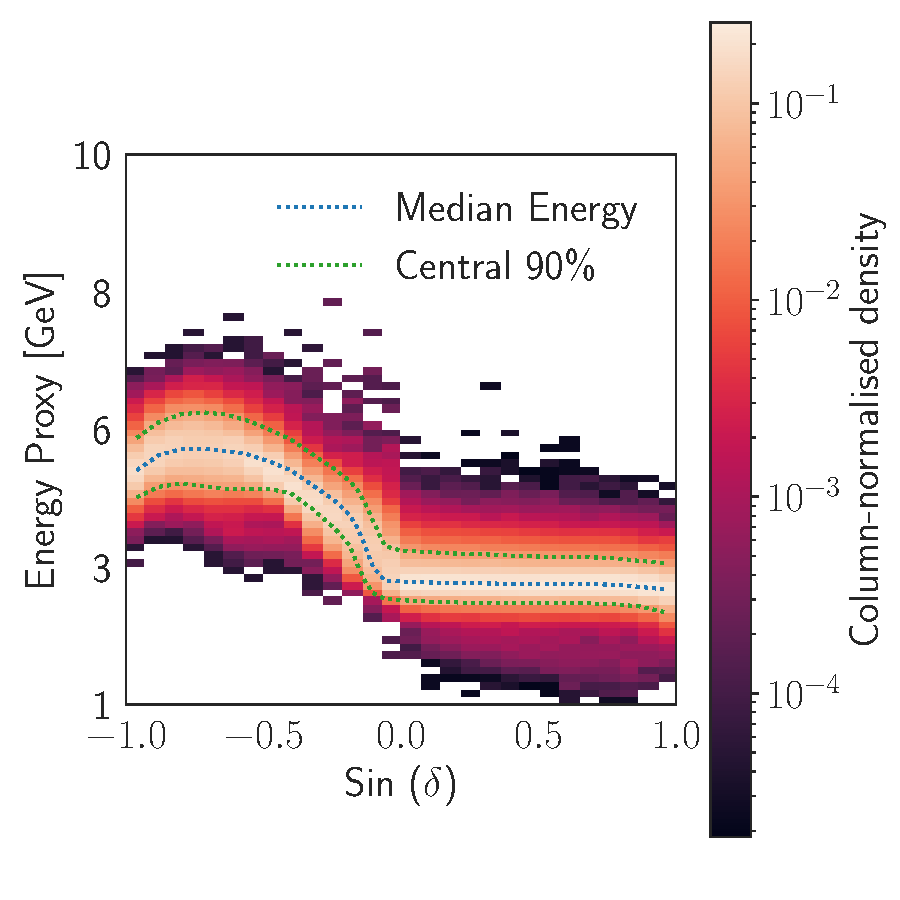
\includegraphics{llh/dec_vs_energy}
	\caption{Background energy proxy distribution, normalised in bins of $\sin(\delta)$.}
	\label{fig:dec_vs_energy}
\end{marginfigure}

In most cases, neutrino energy would be a powerful discriminant between astrophysical signal and atmospheric background. However, in IceCube analysis must be conducted with the observable \emph{Energy Proxy}  ($E_{\textup{proxy}}$), which provides relatively poor energy resolution for through-going tracks (see Chapter N). The normalised energy proxy distribution as a function of $\sin(\delta)$ is given in Figure \ref{fig:dec_vs_energy}, with the median and central 90\% ranges marked by dotted lines. 

It is clear that in the northern hemisphere, this distribution is essentially flat, reflecting the homogeneity of atmospheric neutrino backgrounds in this regime. However, the median energy proxy swiftly increases into the southern hemisphere, as more aggressive cuts are employed to remove the additional atmospheric muon background.

\begin{equation}
\mathcal{B}_{E} (\delta, E_{\textup{proxy}}) = f_{\delta}(E_{\textup{proxy}})
\end{equation}

\subsection{Background Time PDF}

The IceCube detector is characterised by extremely high uptime of >99\%, divided into runs separated by small downtime breaks. Even after processing to final-level event selections, typically consists of livetime at >90\%. The arrival time of background events in Icecube is typically \emph{assumed to be uniform during detector uptime}. This is again only approximately true, as evidenced by Figure \ref{fig:background_rate}.  Six peaks corresponding to winter in the northern hemisphere are clearly visible, corresponding to $\pm \sim5\%$ rate variations.

The atmospheric background rates depend on atmospheric densities which are ultimately temperature-dependent, leading to seasonal variations and clearly-visible annual cycles. This variation is itself an area of scientific interest, being exploited to measure climate with neutrinos CITE. In any case, these effects are partially mitigated in data-based models by the standard method of shuffling measured neutrino arrival times rather than drawing them from PDF. Still, the arrival time anisotropy is a small one.

\begin{equation}
\mathcal{B}_{time} \approx \frac{1}{\textup{livetime}}
\end{equation}

\begin{figure}[!ht]
	\centering 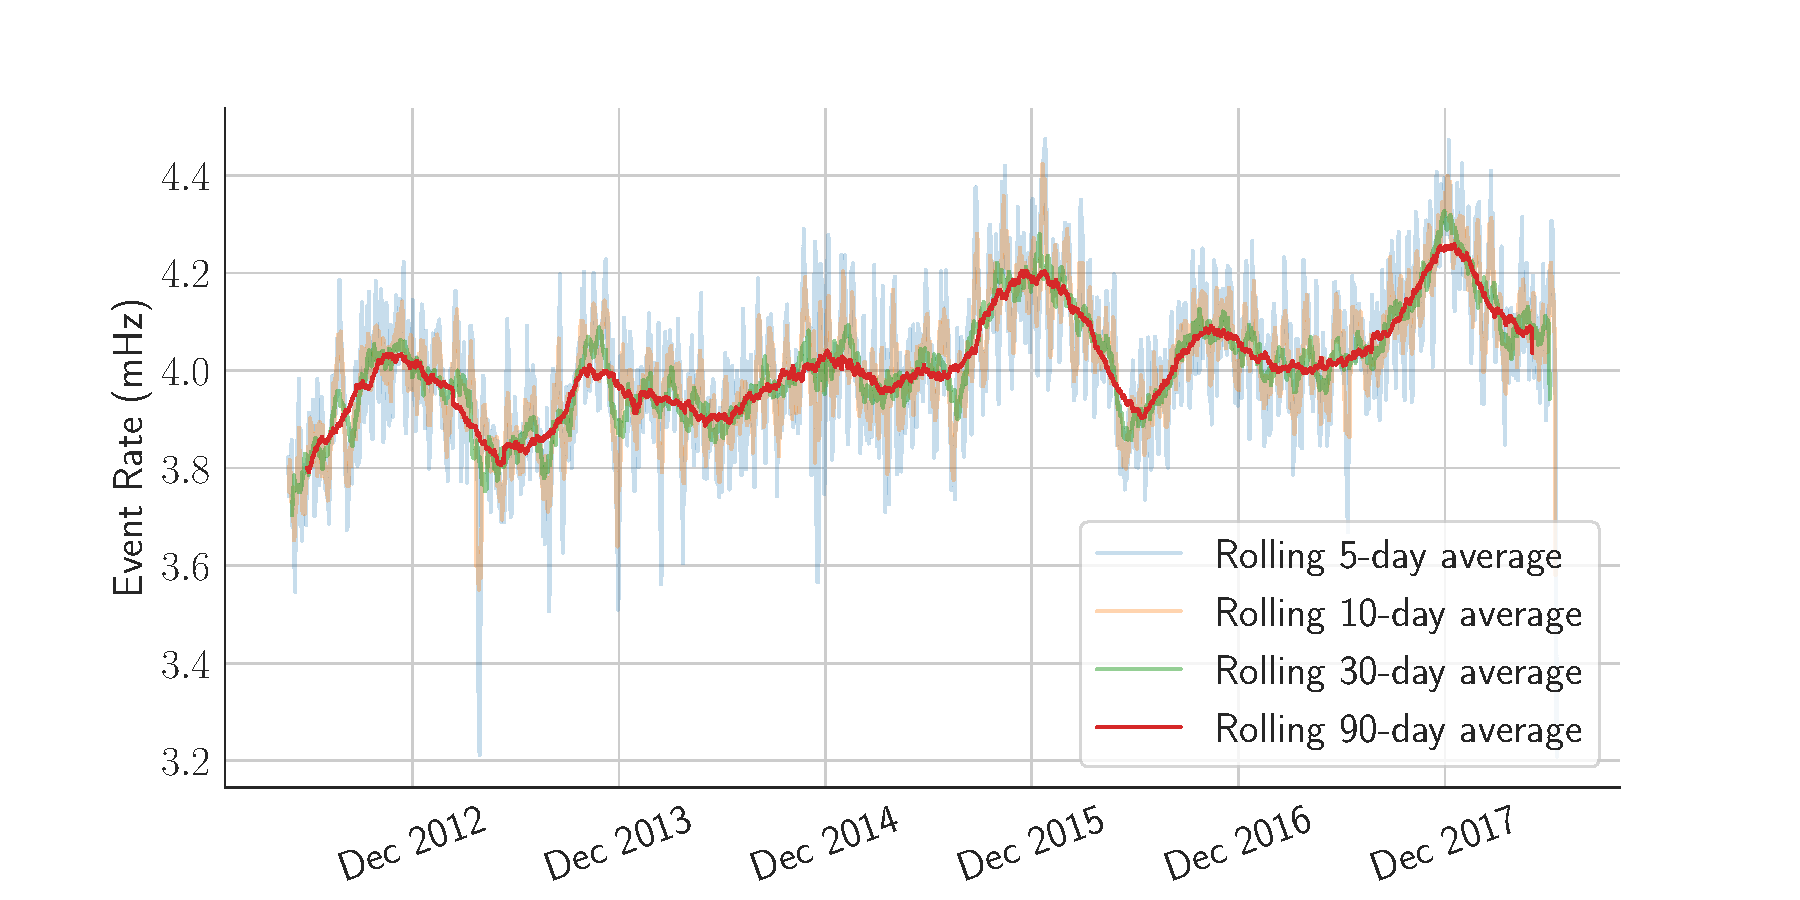
\includegraphics{llh/background_rate}
	\caption{Rolling average of final-level event rate during period of detector uptime.}
	\label{fig:background_rate}
\end{figure}

\section{Signal Hypothesis}

In recognition of the background-dominated regime, signal hypotheses in IceCube are a composite of the null hypothesis with a small number of additional signal-like neutrinos ($n_{s}$). It is assumed that \emph{the total number of neutrino events is essentially fixed by background}, so that N = $n_{s} + n_{b}$. In this case, we define our signal hypothesis as the normalised sum of a background PDF $\mathcal{B}$ and signal PDF $\mathcal{S}$:

\begin{equation}
\mathcal{H}= \frac{n_{s}}{N} \mathcal{S} + \frac{N - n_{s}}{N} \mathcal{B} 
\end{equation}

The signal PDF $\mathcal{S}$ typically describes a single source, or a normalised ensemble of multiple sources. The latter case is known as a \emph{Stacking Analysis}. As for the background, the signal PDF is a product of energy temporal and spatial PDFs

In IceCube, it is common to test a hypotheses that depend on two parameters, $n_{s}$ and $\gamma$. 

\begin{figure}[!ht]
	\centering 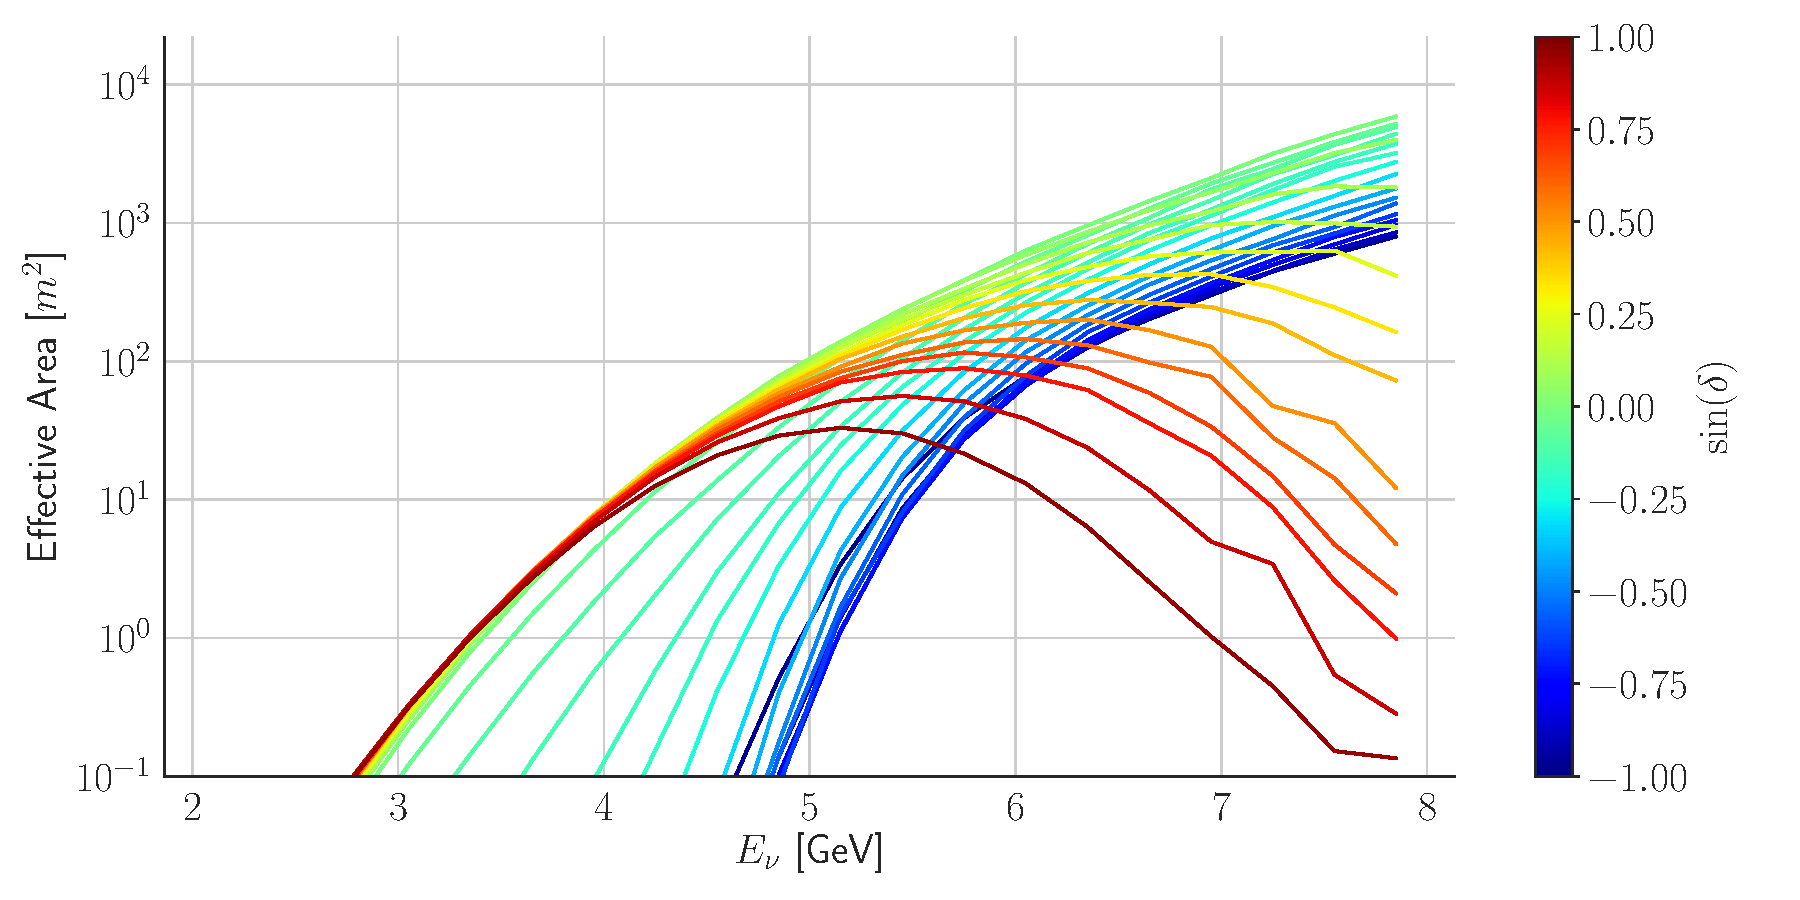
\includegraphics{llh/effective_area}
	\caption{Effective area as a function of neutrino energy and declination.}
	\label{fig:effective_area}
\end{figure}

\subsection{Signal Spatial PDF}

The standard spatial signal PDF is typically stated to be \emph{the assumption a Gaussian PSF centered on the position of a source}. This assumption has been tested extensively in x, and has been found not to describe the data well. Conceptually, even under the limit of a perfect muon track reconstruction, the unmeasurable kinematic angle between the incoming neutrino and outgoing muon will limit the resolution of any search.

However, the performance of directional reconstructions is verified on MC events, and energy-dependent biases in uncertainty estimates are corrected in a process known as pull corrections (see Chapter). So, more precisely, the signal spatial PDF is \emph{assumed to follow the distribution found in baseline MC simulations}, and further \emph{it is assumed that this distribution can be approximated by a circular Gaussian PSF with a single per-event energy-corrected uncertainty parameter}. The former assumption clearly requires that the impact of systematic uncertainties on MC simulation is negligible, but in fact it has been demonstrated that systematic uncertainties are particularly relevant for those high-energy events which are typically 'well-localised' with small estimated uncertainty. The latter assumption was demonstrated to only be valid for these same high-energy events, for which the kinematic angle is negligible. There is thus no regime where both approximations hold well simultaneously.

Spatial prior.

Energy-dependent

It is clear in the left panels of Figure \ref{fig:azimuth_mc} that azimuthal asymmetry is increasingly visible for soft spectra in the northern hemisphere, and approximately  resembles the pattern seen in Figure \ref{fig:azimuth}. However, for both the southern sky and a hard E$^{-1}$ spectrum, there is no such asymmetry. As can be clearly seen in \ref{fig:mc_dec_e}, these corresponds to regimes where the signal is dominated by high-energy events. In general, \emph{the effective area at lower energies is azimuth-dependent, while at higher energies it is approximately uniform}. In any case, as can be seen in the right-hand panels of Figure \ref{fig:azimuth_mc}, the relative discriminating power of azimuth is in all cases substantially less than energy proxy.

\begin{figure}[!ht]
	\centering 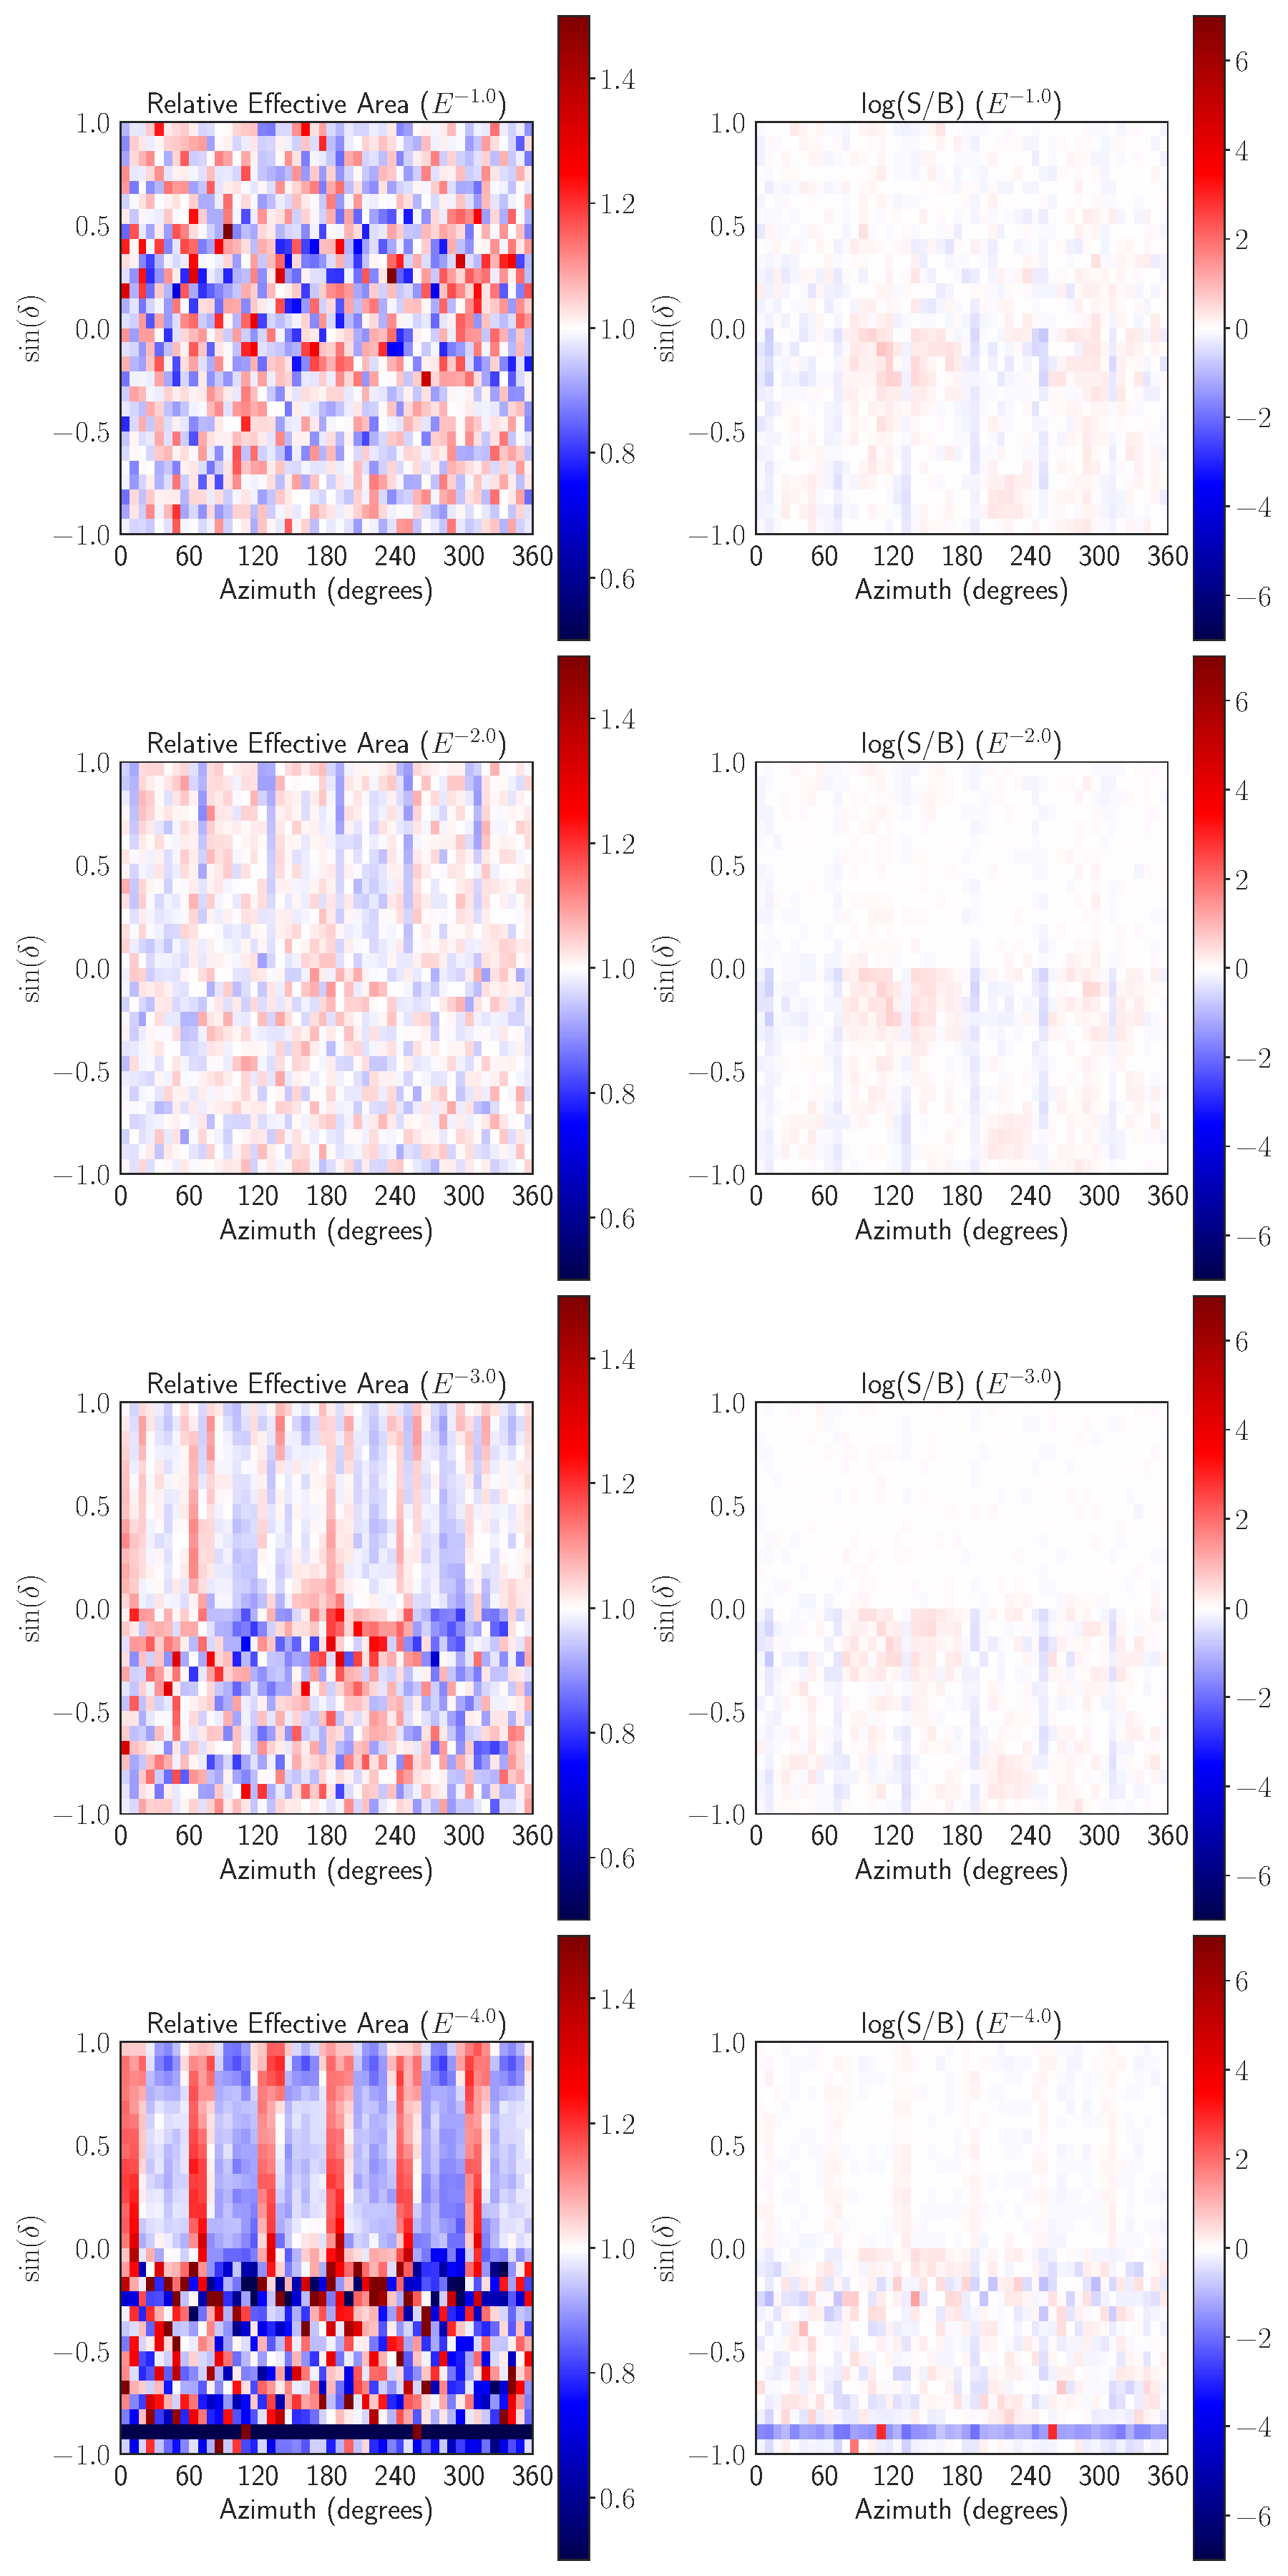
\includegraphics{llh/azimuth_mc}
	\caption{Declination-normalised MC rate as a function of azimuth.}
	\label{fig:azimuth_mc}
\end{figure}

\subsection{Signal Time PDF}

One common assumption for the signal time PDF is a uniform time PDF over a fixed period of livetime. This can be for the entire duration of a dataset, corresponding to a steady neutrino source. This case is typically referred to as a \emph{time-independent analysis}, because it cancels out exactly the assumed background time PDF, yielding a likelihood that does not depend on time. In contrast, transients are typically studied with a \emph{time-dependent analysis} where the signal is assumed to occur over a shorter period than the full data-taking duration. More complex temporal PDFs are possible, such as for periodic sources or models involving exponential-decay-like neutrinos lightcurves.

\subsection{Signal Energy Proxy PDF}

The energy PDF is most commonly \emph{assumed to be an unbroken power extending over the entire energy range of sensitivity for the IceCub detector}, namely from 100 GeV to 10 PeV. This energy spectrum is then convolved with the detector response function through use of weighted MC simulation, yielding an expectated distribution of energy proxy values. Similar to the signal spatial PDF, \emph{it is thus assumed that the baseline MC accurately describes the expected energy proxy distribution}. 

The spectral index, $\gamma$, of the distribution is typically allowed to vary in some range, serving as a parameter which can be fit through a process of maximum likelihood estimation. In other circumstances, a fixed energy PDF is assumed, yielding a fixed energy proxy PDF. An illustration of the expected signal distribution, derived from MC for a range of spectral indices, is illustrated in the left panels Figure \ref{fig:mc_dec_e}.

It is clear that hard spectra result in events with energies substantially above those expected in background, but for softer spectra the distribution narrows and is much more similar to that in Figure \ref{fig:dec_vs_energy}. 

Earth absorption.

Anisotropy!!!

DOMs point down.

\begin{figure}[!ht]
	\centering 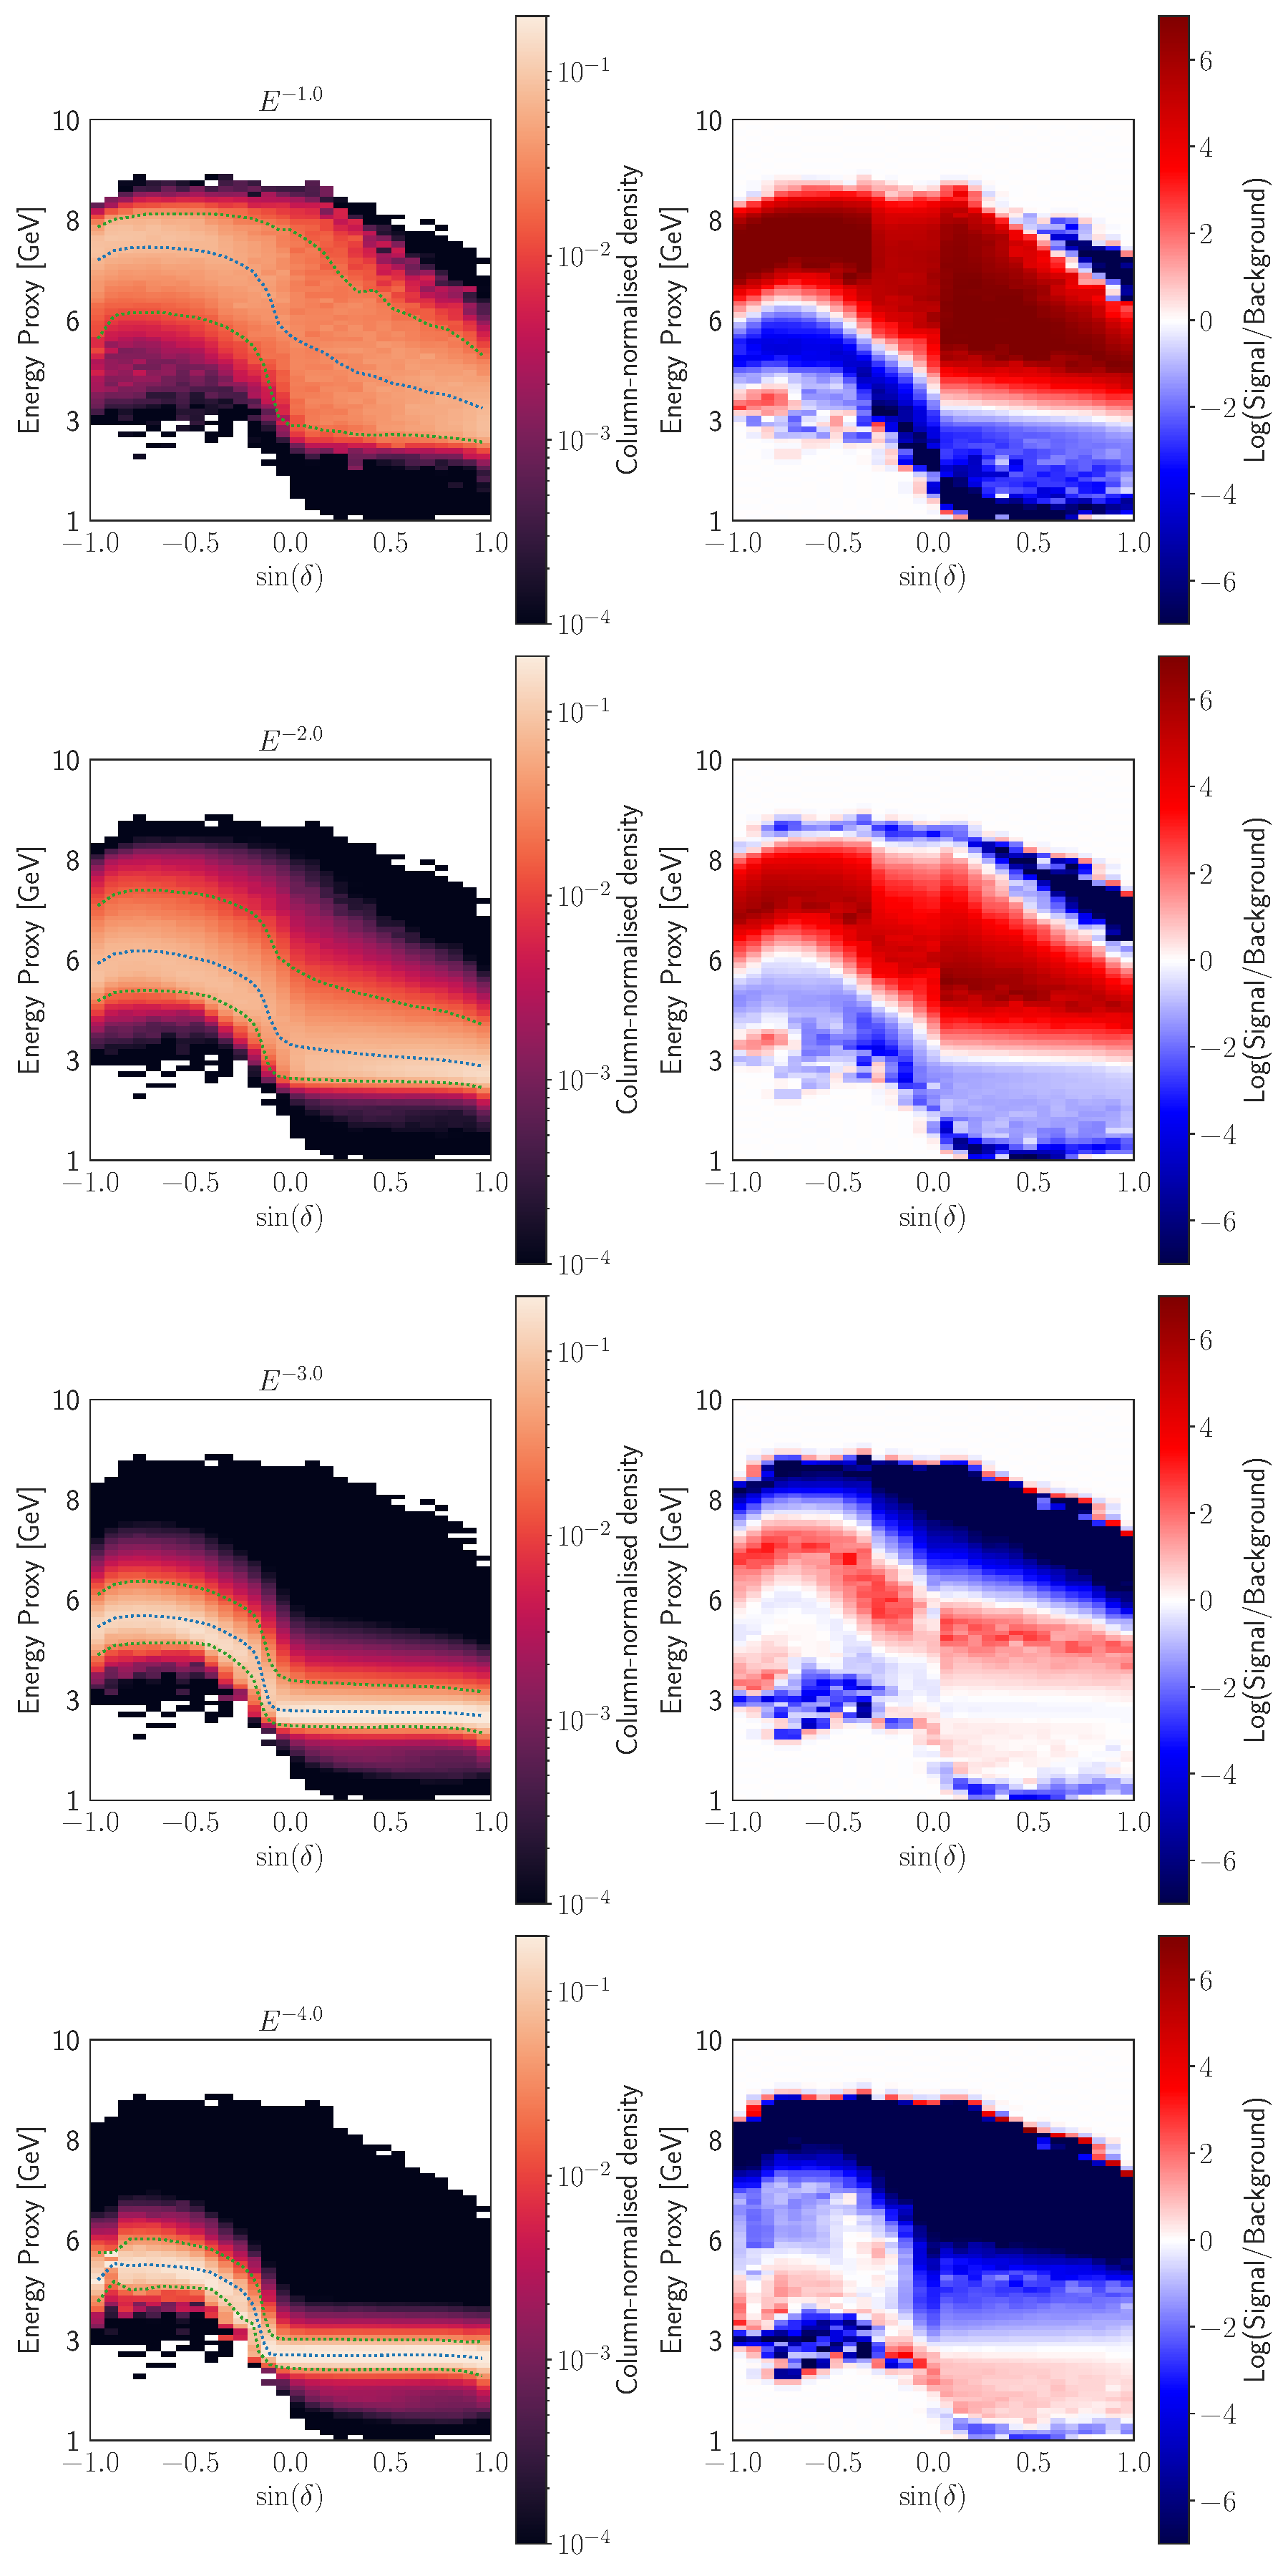
\includegraphics{llh/MC_dec_E}
	\caption{Energy proxy distribution as a function of $\sin(\delta)$, for various signal hypotheses.}
	\label{fig:mc_dec_e}
\end{figure}

\section{Unbinned Likelihood Analysis}
The mathematical formalism outlined above describes a generic approach to likelihood analysis with IceCube. While the approach can be used for a likelihood that is evaluated for discrete regions of parameter space (a \emph{Binned likelihood analysis}), it has long been customary for the likelhood to be evaulated in a continuous event-wise fashion (an \emph{Unbinned likelihood analysis}) citebraun. A likelihood is constructed, and evaluated for each jth individual event, with the overall likelihood given by the product of these N independent datapoints:

\[ \mathcal{L} = \prod_{j}^{N} \mathcal{L}_{j} \]

Ultimately this yields the standard \emph{Point Source Likelihood}:

\[ \mathcal{L}(n_{s}, \gamma) = \prod_{j}^{N} \left(\frac{n_{s}}{N} \mathcal{S}(\theta_{j}, \gamma) + \frac{N - n_{s}}{N} \mathcal{B}(\theta_{j})  \right)\]

We are thus testing a continuum of hypotheses parameterised by $n_{s}$ and $\gamma$, where both $\mathcal{S}$ and $\mathcal{B}$ depend on event-specific observables $\theta_{j}$. These observables are the arrival time, energy proxy, arrival direction and estimated localisation uncertainty. We typically construct the negative log likelihood, and then derive best-fit parameters $\hat{n}_{s}$ and  $\hat{\gamma}$ by a process of maximum likelihood estimation. We take the combination of parameters which maximises the likelihood, and compare this to background expectations using Wilk's Theorum:

\[ TS = 2 \log \left( \frac{ \mathcal{L}(\hat{n}_{s}, \hat{\gamma}) }{\mathcal{L}(n_{s} = 0)} \right)\]

\section{Combining seasons}

yeah, um, seasons

\section{Sensitivity and Discovery Practice}

ndof in practice

\section{Flarestack in practice}

show ns  bias for many many sources

gamma interpolation
mc no data
data no mc

\section{Fitting the relative source weights}

The direct implementation of a well-defined $\mathcal{S}$ for a stacking analysis is the most powerful possible test, \emph{under the assumption that the relative distribution is signal is known}. This condition can be satisfied when a specific model is tested that accurately predicts the relative number of signal events produced by each source in an ensemble. A prediction using multi-wavelength emission as a proxy, or expectations for a population of neutrino standard candles, are common assumptions. However, in an agnostic search for neutrino emission from a source ensemble, the uncertainty of our knowledge should be ideally implemented through priors on our expectations of neutrino emission from each source. The standard \emph{Point Source Likelihood} can be thought of as one extreme with maximum knowledge yielding $\delta$-function priors for the neutrino emission from each source. The other extreme is one of maximum ignorance, in which flat priors $n_{s, k}$ for each kth source is allowed to vary completely independently. In that case, we have a \emph{multi-source likelihood}:

\[ \mathcal{L}(n_{s}, \gamma) = \prod_{j}^{N} \left(\sum_{k} \left[ \frac{n_{s, k}}{N} \mathcal{S}_{k}(\theta_{j}, \gamma) \right]+ \frac{N - \sum_{k} \left[ n_{s, k} \right] }{N} \mathcal{B}(\theta_{j})  \right)\]

This approach is commonly referred to as \emph{fitting the weights} of each source, in contrast to the standard method of \emph{fixed source weights}. Additional flexibility comes at the expense of more independent fit parameters, and thus a higher TS threshold to achieve fixed significance. In the limit of many sources, each with sub-unity neutrino expectations, the number of degrees of freedom would exceed the number of expected signal events. It is most useful for analysing a small number of sources, in which the relative neutrino distribution is not known, but for which 

A more realistic intermediate approach, in which non-flat priors quantify our expectations in the possible neutrino emission variation between sources, would likely offer some additional improvement over both methods. 

\section{Penalty Factors}
lalala, use misc graphic

\begin{figure}[!ht]
	\centering 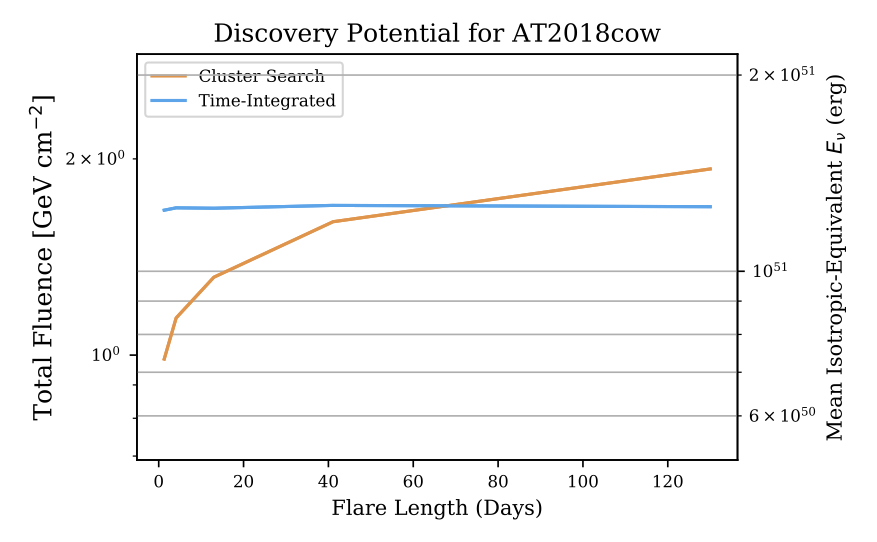
\includegraphics{results/flare_vs_box_disc}
	\caption{The $5\sigma$ Discovery Potential for AT2018cow, in both total fluence and isotropic-equivalent energy, as a function of flare length. The analysis tests flares within a pre-defined 130 day window. For flares much shorter than the search window, significantly less fluence is required to make a discovery with the cluster-search than for a time-integrated analysis.}
	\label{fig:DiscTime}
\end{figure}

\section{Shortcuts to likelihood minimisation}
The evaulation of this likelihood is time-consuming, and the implementation of this process in \emph{\href{https://github.com/IceCubeOpenSource/flarestack}{Flarestack}} makes several additional simplifications to speed calculations. 

cite alex, skylab

The first is the recognition that the parameters which maximise the likelihood will also maximise the likelihood ratio, and thus the test statistic. Rather than evaluating two independent likelihoods, we can instead directly evaluate the test statistic:

\begin{equation}
	TS = 2 \log \left( \frac{ \mathcal{L}(\hat{n}_{s}, \hat{\gamma}) }{\mathcal{L}(n_{s} = 0)} \right)
\end{equation}
\begin{equation}
TS = 2 \log  \frac{\prod_{j}^{N} \left(\frac{n_{s}}{N} \mathcal{S}(\theta_{j}, \gamma) + \frac{N - n_{s}}{N} \mathcal{B}(\theta_{j})  \right)}{\prod_{j}^{N}\mathcal{B}(\theta_{j})}
\end{equation}

By dividing this through, we find: 

\begin{equation}
	TS =  2 \log \left(  \prod_{j}^{N} \left(\frac{n_{s}}{N} \left[\frac{\mathcal{S}(\theta_{j}, \gamma)}{\mathcal{B}(\theta_{j})} \right] + 1 - \frac{n_{s}}{N} \right) \right) 
\end{equation}
\begin{equation}
	TS = 2 \sum_{j}^{N} \log \left(\frac{n_{s}}{N} \left[ \frac{\mathcal{S}(\theta_{j}, \gamma)}{\mathcal{B}(\theta_{j}) } - 1 \right] + 1 \right) 
\label{eq:TS_reduced}
\end{equation}

Equation \ref{eq:TS_reduced}  is faster to evaluate, because it bypasses the need to calculate both signal and background energy proxy PDFs explicitly. Instead, we can precomputing the ratio $\frac{\mathcal{S}}{\mathcal{B}}$ for a variety of spectral indices, saving a per-event division calculation.

An additional simplifying assumption is that neutrinos are typically localised to a resolution of $\sim$1 degree, so events which lie many degrees from a source have a negligible probability of being signal. For events lying more than 5 degrees away, and those within 5 degrees but with a spatial likelihood ratio less than x, we make the approximation that $\mathcal{S} \approx 0$ so then $TS \approx 0$. Using the formulation in Equation \ref{eq:TS_reduced} , we see we can simply neglect to evaluate the likelihood for these events, without altering the final sum. This box cut thus removes the overwhelming majority of events from the likelihood evaluation step, yielding vast speed improvements while having a negligible impact on the fitting process.
\section{Trial correction}


The trial factor corresponds to the number of independent hypotheses that were tested. It is a common misconception that the trial factor is particularly important for cases when two hypotheses are similar. In the limit that two hypotheses are so similar as to be essentially identical, then would be no need for a trial correction at all, since the test statistic for each would be identical. The trial factor should correct the degree to which hypotheses are capable of giving multiple independent TS values.
